\section{Performance Evaluation}

\subsection{Parameter Settings}
\begin{figure}[t]
    \centering
    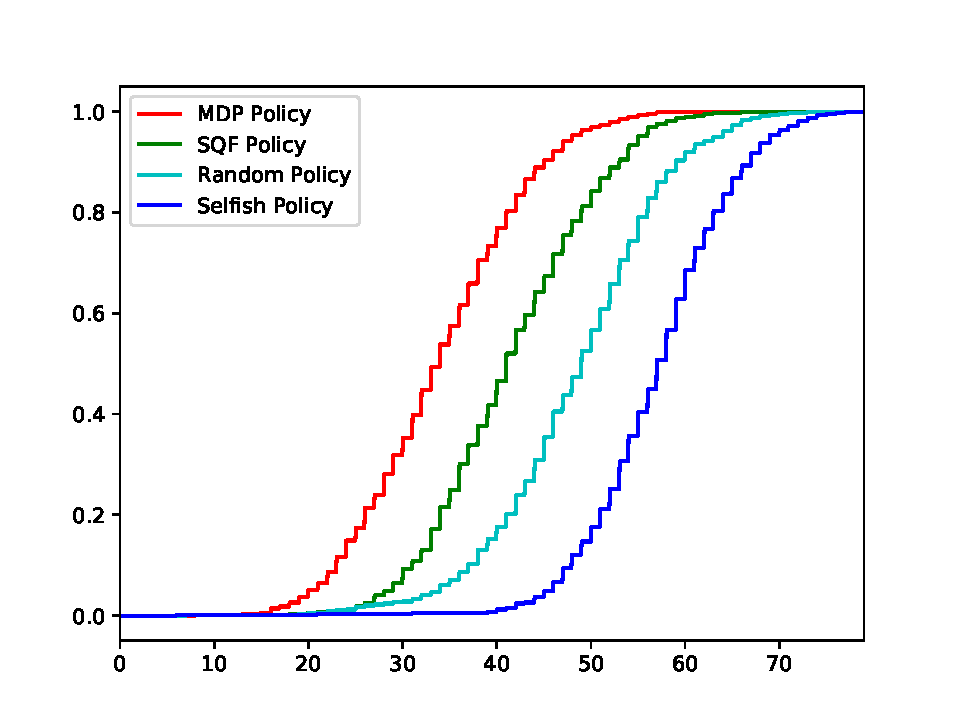
\includegraphics[width=0.80\textwidth]{images/535_ul_cmp_proc_LargeDelay_cdf.pdf}
    \caption{An example with 5 APs and 3 edge servers, when the \brlatency~is large.}
    \label{fig:eval_general}
\end{figure}

\begin{itemize}
    \item $K=5$ AP nodes, $M=3$ ES nodes, and $J=5$ types of jobs;
    \item Each time slot with $\tau=0.05$ s (a.k.a $50$ ms), and broadcast interval $T=N \cdot \tau$ with $N=30$;
    \item The maximum uploading time is $\Xi = 3 T$, and the \brlatency is shorter than $t_B$;
    \item (arrival rate is random generated as $\lambda_{k,j} \ll 1/N$)
    \item job processing time distribution generated from real data trace;
    \item Each queue on ES with maximum 10 jobs.
\end{itemize}

We compare the proposed algorithm with other 3 heuristic algorithms.
Compared Algorithm:
\begin{itemize}
    \item \textbf{Random Dispatching Policy}:
            randomly dispatch jobs to edge servers;
    \item \textbf{Local Greedy Algorithm (baseline policy)}:
            always choose the minimum processing time server for the job, and not queue-aware; this policy is taken as initial baseline policy as the start of our proposed algorithm;
    \item \textbf{Local Queue-aware Greedy Algorithm}:
            always choose the queue with minimum queue length while the obtained queue state is stale;
    \item \textbf{Mixed Queue-aware Greedy Algorithm}:
            mixed the above two algorithm with weight factor $\alpha = 0.5$;
\end{itemize}

% [abandon, cause useless]
% \subsection{Estimation Error Analysis}
% (If these graphs are not good, they are not going to appear on final draft.)
% \begin{itemize}
%     \item Two curves, one for real cost against time slot, one for expected sampling cost against time intervals; (if the accumulate area within the latter one has little/bounded error with real cost, then it's okay and the correctness is support by simulation)
%     \item 
% \end{itemize}

\subsection{Performance Analysis}
Compared with different parameter settings:
\begin{itemize}
    \item CDF of cost (Average JCT), with different broadcast $t_B$ setting;
    \item CDF of cost (Average JCT), with different \brlatency $D_{i,k}$ setting;
\end{itemize}

Compared with other algorithms:
\begin{itemize}
    \item CDF of cost (Average JCT);
    \item CDF of queue length;
    \item CDF of \# of dropped jobs (over the queue limit);
\end{itemize}